% Lecture 1: Course Overview and Python Environment Setup
% 75 slides for 3-hour presentation
\documentclass[aspectratio=169,10pt]{beamer}

% Essential packages
\usepackage[utf8]{inputenc}
\usepackage[T1]{fontenc}
\usepackage{amsmath,amssymb,amsthm}
\usepackage{graphicx}
\usepackage{listings}
\usepackage{xcolor}
\usepackage{tikz}
\usepackage{algorithm}
\usepackage{algorithmic}
\usepackage{hyperref}
\usetikzlibrary{arrows.meta,positioning} % 최신 권장
\tikzset{>={Stealth[length=2.5mm]}}      % 전역 화살표 팁
% Use mimic.sty to prevent overfull boxes
\usepackage{mimic}

% Theme
\usetheme{Madrid}
\usecolortheme{seahorse}
\setbeamertemplate{navigation symbols}{}
\setbeamertemplate{footline}[frame number]

% Code listing settings
\lstset{
    language=Python,
    basicstyle=\ttfamily\scriptsize,
    keywordstyle=\color{blue}\bfseries,
    stringstyle=\color{red},
    commentstyle=\color{green!60!black},
    showstringspaces=false,
    breaklines=true,
    breakatwhitespace=true,
    frame=single,
    numbers=left,
    numberstyle=\tiny\color{gray},
    xleftmargin=1em,
    framexleftmargin=1em
}

% Title page information
\title{Reinforcement Learning}
\subtitle{Lecture 1: Course Overview and Environment Setup}
\author{Taehoon Kim}
\institute{Sogang University MIMIC Lab \\ \url{https://mimic-lab.com}}
\date{Fall Semester 2025}

\begin{document}

% Slide 1: Title
\frame{\titlepage}

% Slide 3: Learning Objectives
\begin{frame}{Learning Objectives}
\begin{block}{By the end of this lecture, you will:}
\begin{itemize}
    \item Understand the relationship among AI, ML, and RL
    \item Master the MDP formalism and core RL notation
    \item Set up a reproducible PyTorch 2.x environment
    \item Implement the standard code header for the course
    \item Complete 9 hands-on experiments
    \item Pass the integrated smoke test
\end{itemize}
\end{block}

\begin{alertblock}{Prerequisites}
\begin{itemize}
    \item Python programming experience
    \item Basic linear algebra and calculus
    \item Familiarity with neural networks (helpful)
\end{itemize}
\end{alertblock}
\end{frame}

% Section 1: Course Overview (Slides 4-20)
\section{Course Overview}

% Slide 4: AI-ML-RL Hierarchy
\begin{frame}{The AI-ML-RL Hierarchy}
\begin{center}
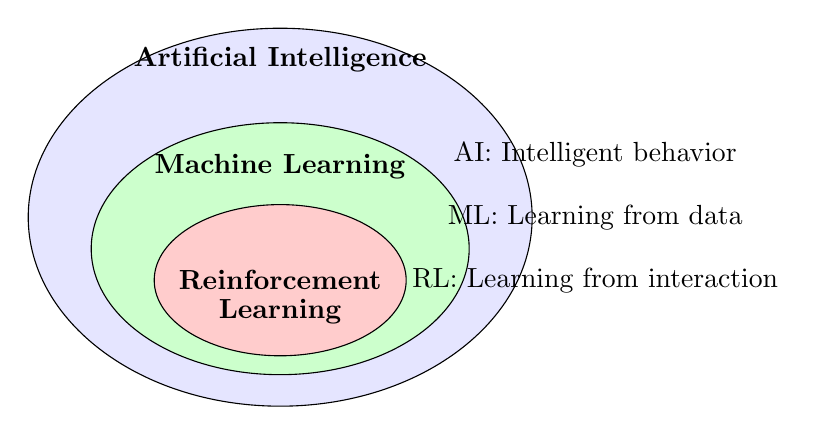
\begin{tikzpicture}[scale=0.8]
    \draw[fill=blue!10] (0,0) ellipse (4cm and 3cm);
    \node at (0,2.5) {\textbf{Artificial Intelligence}};
    
    \draw[fill=green!20] (0,-0.5) ellipse (3cm and 2cm);
    \node at (0,0.8) {\textbf{Machine Learning}};
    
    \draw[fill=red!20] (0,-1) ellipse (2cm and 1.2cm);
    \node at (0,-1) {\textbf{Reinforcement}};
    \node at (0,-1.5) {\textbf{Learning}};
    
    \node[align=left] at (5,1) {AI: Intelligent behavior};
    \node[align=left] at (5,0) {ML: Learning from data};
    \node[align=left] at (5,-1) {RL: Learning from interaction};
\end{tikzpicture}
\end{center}
\end{frame}

% Slide 5: What is Reinforcement Learning?
\begin{frame}{What is Reinforcement Learning?}
\begin{columns}
\column{0.5\textwidth}
\begin{center}
\begin{block}{Definition}
RL learns optimal behavior through \textbf{trial and error} interaction with an environment
\end{block}

\begin{itemize}
    \item Agent takes actions
    \item Environment provides rewards
    \item Goal: maximize cumulative reward
    \item No explicit supervision
\end{itemize}
\end{center}
\column{0.5\textwidth}
\begin{center}
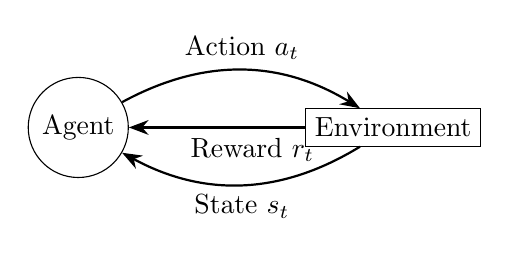
\begin{tikzpicture}[scale=1.0]
    \node[draw,circle] (A) at (0,0) {Agent};
    \node[draw,rectangle] (E) at (4,0) {Environment};
    
    \draw[->,thick] (A) to[bend left=30] node[above] {Action $a_t$} (E);
    \draw[->,thick] (E) to[bend left=30] node[below] {State $s_t$} (A);
    \draw[->,thick] (E) to node[below,pos=0.3] {Reward $r_t$} (A);
\end{tikzpicture}
\end{center}
\end{columns}
\end{frame}

% Slide 6: RL vs Supervised Learning
\begin{frame}{RL vs Supervised Learning}
\begin{table}
\centering
\small
\begin{tabular}{|l|l|l|}
\hline
\textbf{Aspect} & \textbf{Supervised} & \textbf{Reinforcement} \\
\hline
Feedback & Immediate labels & Delayed rewards \\
Data & i.i.d. samples & Sequential, correlated \\
Exploration & Not needed & Essential \\
Goal & Minimize error & Maximize return \\
Training & Offline, batch & Online, interactive \\
\hline
\end{tabular}
\end{table}

\begin{block}{Key Insight}
RL faces the \textbf{exploration-exploitation dilemma}: 
Should the agent try new actions (explore) or stick with known good actions (exploit)?
\end{block}
\end{frame}

% Slide 7: Course Structure
\begin{frame}{13-Week Course Structure}
\begin{columns}
\column{0.5\textwidth}
\textbf{Foundations (Weeks 1-4)}
\begin{itemize}
    \item Week 1: Environment Setup
    \item Week 2: Deep Learning Essentials
    \item Week 3: RL Fundamentals
    \item Week 4: Mathematical Foundations
\end{itemize}

\textbf{Value-Based (Weeks 5-7)}
\begin{itemize}
    \item Week 5: Q-Learning
    \item Week 6: Deep Q-Networks
    \item Week 7: DQN Project
\end{itemize}

\column{0.5\textwidth}
\textbf{Policy-Based (Weeks 8-10)}
\begin{itemize}
    \item Week 8: Policy Gradients
    \item Week 9: Actor-Critic Methods
    \item Week 10: PPO
\end{itemize}

\textbf{Advanced (Weeks 11-13)}
\begin{itemize}
    \item Week 11: Current Trends
    \item Week 12: Project Development
    \item Week 13: Final Presentations
\end{itemize}
\end{columns}
\end{frame}


% Slide 10: Required Tools
\begin{frame}{Required Tools and Resources}
\begin{columns}
\column{0.5\textwidth}
\textbf{Software}
\begin{itemize}
    \item Python 3.10-3.12
    \item PyTorch 2.x
    \item Gymnasium
    \item TensorBoard
    \item Jupyter/Colab
    \item Git
\end{itemize}

\column{0.5\textwidth}
\textbf{Hardware}
\begin{itemize}
    \item CPU: Any modern processor
    \item GPU: Optional but recommended
    \item RAM: 8GB minimum
    \item Storage: 20GB free space
\end{itemize}
\end{columns}

\begin{alertblock}{Cloud Alternative}
Google Colab provides free GPU access - all experiments will run there
\end{alertblock}
\end{frame}

% Section 2: Mathematical Foundations (Slides 11-25)
\section{Mathematical Foundations}

% Slide 11: Section Overview
\begin{frame}{Mathematical Foundations}
\begin{center}
\Large{Understanding the MDP Framework}
\end{center}

\begin{block}{Topics}
\begin{itemize}
    \item Markov Decision Processes (MDPs)
    \item States, Actions, and Rewards
    \item Policies and Value Functions
    \item Bellman Equations
    \item Optimality Conditions
\end{itemize}
\end{block}
\end{frame}

% Slide 12: MDP Definition
\begin{frame}{Markov Decision Process (MDP)}
An MDP is defined as a tuple $\mathcal{M} = (\mathcal{S}, \mathcal{A}, \mathcal{P}, r, \gamma)$:

\begin{itemize}
    \item $\mathcal{S}$: State space
    \item $\mathcal{A}$: Action space
    \item $\mathcal{P}(s'|s,a)$: Transition probability
    \item $r(s,a)$: Reward function
    \item $\gamma \in [0,1)$: Discount factor
\end{itemize}

\begin{block}{Markov Property}
The future depends only on the current state, not the history:
$$P(S_{t+1}|S_t, A_t, S_{t-1}, A_{t-1}, ...) = P(S_{t+1}|S_t, A_t)$$
\end{block}
\end{frame}

% Slide 13: Episode Structure
\begin{frame}{Episode Structure}
An episode is a sequence of interactions:
$$(S_0, A_0, R_1, S_1, A_1, R_2, ..., S_{T-1}, A_{T-1}, R_T, S_T)$$

\begin{center}
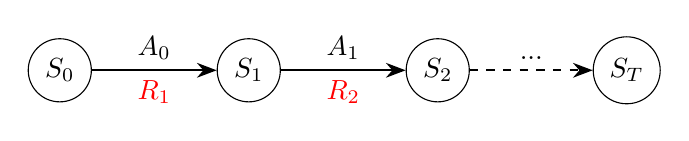
\begin{tikzpicture}[scale=0.8]
    \node[draw,circle] (s0) at (0,0) {$S_0$};
    \node[draw,circle] (s1) at (3,0) {$S_1$};
    \node[draw,circle] (s2) at (6,0) {$S_2$};
    \node[draw,circle] (st) at (9,0) {$S_T$};
    
    \draw[->,thick] (s0) to node[above] {$A_0$} node[below,red] {$R_1$} (s1);
    \draw[->,thick] (s1) to node[above] {$A_1$} node[below,red] {$R_2$} (s2);
    \draw[->,thick,dashed] (s2) to node[above] {...} (st);
\end{tikzpicture}
\end{center}

Terminal state $S_T$ ends the episode
\end{frame}

% Slide 14: Return Definition
\begin{frame}{Return and Discounting}
The \textbf{return} $G_t$ is the cumulative discounted reward:
$$G_t = \sum_{k=0}^{\infty} \gamma^k R_{t+k+1}$$

\begin{block}{Why Discounting?}
\begin{itemize}
    \item Mathematical convenience (convergence)
    \item Uncertainty about the future
    \item Preference for immediate rewards
\end{itemize}
\end{block}

\begin{example}
If $\gamma = 0.9$ and rewards are $[1, 2, 3, ...]$:
$$G_0 = 1 + 0.9 \cdot 2 + 0.81 \cdot 3 + ... = 10$$
\end{example}
\end{frame}

% Slide 15: Policy Definition
\begin{frame}{Policy}
A \textbf{policy} $\pi$ defines the agent's behavior:
$$\pi(a|s) = P(A_t = a | S_t = s)$$

\begin{columns}
\column{0.5\textwidth}
\textbf{Deterministic Policy}
$$a = \pi(s)$$
One action per state

\column{0.5\textwidth}
\textbf{Stochastic Policy}
$$\pi(a|s) \in [0,1]$$
Probability distribution over actions
\end{columns}

\begin{block}{Goal}
Find the optimal policy $\pi^*$ that maximizes expected return:
$$J(\pi) = \mathbb{E}_{\pi}\left[\sum_{t=0}^{\infty} \gamma^t R_{t+1}\right]$$
\end{block}
\end{frame}

% Slide 16: Value Functions
\begin{frame}{Value Functions}
\begin{block}{State Value Function}
Expected return starting from state $s$ following policy $\pi$:
$$v^{\pi}(s) = \mathbb{E}_{\pi}[G_t \mid S_t = s]$$
\end{block}

\begin{block}{Action Value Function (Q-function)}
Expected return starting from state $s$, taking action $a$, then following $\pi$:
$$q^{\pi}(s,a) = \mathbb{E}_{\pi}[G_t \mid S_t = s, A_t = a]$$
\end{block}

\textbf{Relationship:} \\
The policy $\pi(a|s)$ is a probability distribution over actions given state $s$. 
Therefore, the state value is the expected action value under this distribution:
$$v^{\pi}(s) = \sum_{a \in \mathcal{A}} \pi(a|s) \cdot q^{\pi}(s,a)$$
\end{frame}

% Slide 17: Bellman Equations
\begin{frame}{Bellman Equations}
Value functions satisfy recursive relationships:

\begin{block}{Bellman Expectation Equation}
$$v^{\pi}(s) = \sum_a \pi(a|s) \sum_{s'} \mathcal{P}(s'|s,a)[r(s,a) + \gamma v^{\pi}(s')]$$
\end{block}

\begin{block}{Bellman Optimality Equation}
$$v^*(s) = \max_a \sum_{s'} \mathcal{P}(s'|s,a)[r(s,a) + \gamma v^*(s')]$$
\end{block}

These equations are the foundation for RL algorithms!
\end{frame}

% Slide: Bellman Equations (Detailed Explanation)
\begin{frame}{Bellman Equations: Detailed Explanation}

\begin{block}{Bellman Expectation Equation}
\begin{itemize}
    \item Under a given policy $\pi$, the value of a state $s$ is
    \item the weighted sum of possible actions, where weights are given by $\pi(a|s)$.
    \item Each action leads probabilistically to a next state $s'$ according to $\mathcal{P}(s'|s,a)$, yielding an immediate reward $r(s,a)$.
    \item Therefore, $v^\pi(s)$ is the expected immediate reward plus the discounted value of the next state.
\end{itemize}
\end{block}

\begin{block}{Bellman Optimality Equation}
\begin{itemize}
    \item For the optimal policy, the value of state $s$ is
    \item the maximum expected return achievable over all possible actions.
    \item Instead of averaging with $\pi(a|s)$, we take $\max_a$.
    \item Solving this recursive relation gives the optimal value function $v^*(s)$ and the optimal policy.
\end{itemize}
\end{block}

\begin{center}
\textit{Key idea: The Bellman equations express the value of a state as a recursive relationship between immediate reward and future value.}
\end{center}
\end{frame}

% Slide: Bellman — Expectation vs Optimality with one GridWorld
\begin{frame}{Bellman: Expectation vs Optimality (GridWorld)}

\begin{columns}[T,onlytextwidth]
%==================== Left: Expectation ====================
\begin{column}{0.49\textwidth}
\centering
\textit{Expectation (policy evaluation)}

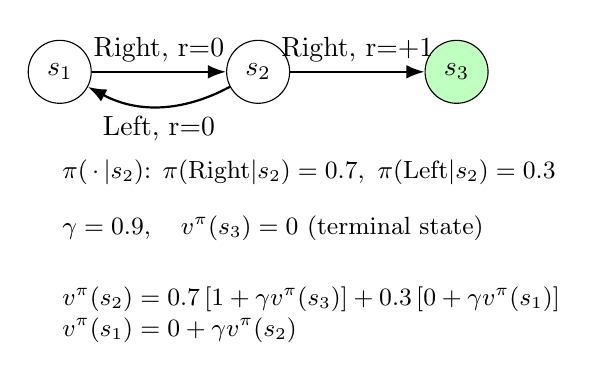
\begin{tikzpicture}[scale=0.9, >=Latex, node distance=2.6cm]
  % Nodes
  \node[draw,circle,minimum size=8mm] (s1) at (0,0) {$s_1$};
  \node[draw,circle,minimum size=8mm] (s2) at (2.8,0) {$s_2$};
  \node[draw,circle,fill=green!25,minimum size=8mm] (s3) at (5.6,0) {$s_3$};

  % Transitions
  \draw[->,thick] (s1) -- node[above] {Right, r=0} (s2);
  \draw[->,thick] (s2) -- node[above] {Right, r=+1} (s3);
  \draw[->,thick] (s2) to[bend left=28] node[below] {Left, r=0} (s1);

  % Policy probabilities at s2
  \node[draw=none,anchor=north west,font=\small] at (-0.1,-1.1)
       {$\pi(\,\cdot\,|s_2)$: $\pi(\text{Right}|s_2)=0.7,\ \pi(\text{Left}|s_2)=0.3$};
  \node[draw=none,anchor=north west,font=\small] at (-0.1,-1.9)
       {$\gamma=0.9,\quad v^\pi(s_3)=0$ (terminal state)};

  % Value update snippet
  \node[draw=none,anchor=north west,font=\small,align=left] at (-0.1,-2.9)
       {$v^\pi(s_2)=0.7\,[1+\gamma v^\pi(s_3)] + 0.3\,[0+\gamma v^\pi(s_1)]$\\
        $v^\pi(s_1)=0+\gamma v^\pi(s_2)$};
\end{tikzpicture}

\end{column}
%==================== Right: Optimality ====================
\begin{column}{0.49\textwidth}
\centering
\textit{Optimality (control)}

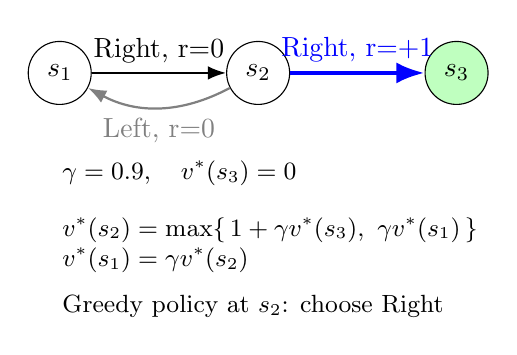
\begin{tikzpicture}[scale=0.9, >=Latex, node distance=2.6cm]
  % Nodes
  \node[draw,circle,minimum size=8mm] (s1) at (0,0) {$s_1$};
  \node[draw,circle,minimum size=8mm] (s2) at (2.8,0) {$s_2$};
  \node[draw,circle,fill=green!25,minimum size=8mm] (s3) at (5.6,0) {$s_3$};

  % Transitions, highlight the greedy edge
  \draw[->,thick] (s1) -- node[above] {Right, r=0} (s2);
  \draw[->,ultra thick,blue] (s2) -- node[above] {Right, r=+1} (s3);
  \draw[->,thick,gray] (s2) to[bend left=28] node[below,gray] {Left, r=0} (s1);

  % Optimal update
  \node[draw=none,anchor=north west,font=\small] at (-0.1,-1.1)
       {$\gamma=0.9,\quad v^*(s_3)=0$};
  \node[draw=none,anchor=north west,font=\small,align=left] at (-0.1,-1.9)
       {$v^*(s_2)=\max\{\,1+\gamma v^*(s_3),\ \gamma v^*(s_1)\,\}$\\
        $v^*(s_1)=\gamma v^*(s_2)$};
  \node[draw=none,anchor=north west,font=\small,align=left] at (-0.1,-3.0)
       {Greedy policy at $s_2$: choose Right};
\end{tikzpicture}

\end{column}
\end{columns}

\medskip
\centering
\small Expectation averages action values using $\pi(a|s)$, while Optimality takes the maximum over actions.
\end{frame}

% Slide 18: Optimal Policy
\begin{frame}{Optimal Policy and Value Functions}
\begin{itemize}
    \item Optimal value function: $v^*(s) = \max_{\pi} v^{\pi}(s)$
    \item Optimal Q-function: $q^*(s,a) = \max_{\pi} q^{\pi}(s,a)$
    \item Optimal policy: $\pi^*(a|s) = \arg\max_a q^*(s,a)$
\end{itemize}

\begin{theorem}[Policy Improvement]
For any policy $\pi$, the greedy policy with respect to $v^{\pi}$ is at least as good as $\pi$
\end{theorem}

This leads to \textbf{policy iteration} and \textbf{value iteration} algorithms
\end{frame}

% Slide: Policy Improvement Intuition (with spacing fixed)
\begin{frame}{Policy Improvement Intuition}

\begin{columns}[T,onlytextwidth]
%==================== Left: Current Policy ====================
\begin{column}{0.5\textwidth}
\centering
\textit{Current policy $\pi$ (mixed actions)}

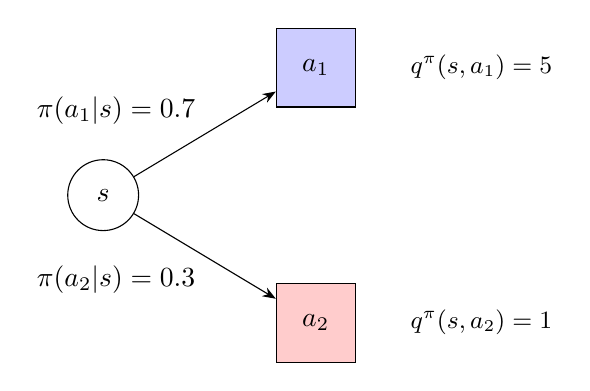
\begin{tikzpicture}[scale=0.9, >=Stealth, node distance=3.5cm]
  % State
  \node[draw,circle,minimum size=9mm] (s) at (0,0) {$s$};

  % Actions
  \node[draw,rectangle,minimum size=10mm,fill=blue!20] (a1) at (3,1.8) {$a_1$};
  \node[draw,rectangle,minimum size=10mm,fill=red!20]  (a2) at (3,-1.8) {$a_2$};

  % Edges
  \draw[->] (s) -- (a1) node[midway,above left] {$\pi(a_1|s)=0.7$};
  \draw[->] (s) -- (a2) node[midway,below left] {$\pi(a_2|s)=0.3$};

  % Q-values
  \node[draw=none,anchor=west,font=\small] at (4.2,1.8) {$q^\pi(s,a_1)=5$};
  \node[draw=none,anchor=west,font=\small] at (4.2,-1.8) {$q^\pi(s,a_2)=1$};
\end{tikzpicture}

\vspace{3pt}

\[
v^\pi(s) = 0.7 \times 5 + 0.3 \times 1 = 3.8
\]
\end{column}

%==================== Right: Greedy Policy ====================
\begin{column}{0.5\textwidth}
\centering
\textit{Greedy policy $\pi'$ (choose best action)}

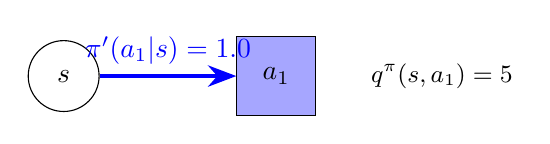
\begin{tikzpicture}[scale=0.9, >=Stealth, node distance=3.5cm]
  % State
  \node[draw,circle,minimum size=9mm] (s) at (0,0) {$s$};

  % Best action
  \node[draw,rectangle,minimum size=10mm,fill=blue!35] (a1) at (3,0) {$a_1$};

  % Edge
  \draw[->,ultra thick,blue] (s) -- (a1) node[midway,above] {$\pi'(a_1|s)=1.0$};

  % Q-value
  \node[draw=none,anchor=west,font=\small] at (4.2,0) {$q^\pi(s,a_1)=5$};
\end{tikzpicture}

\vspace{6pt}

\[
v^{\pi'}(s) = \max_a q^\pi(s,a) = 5
\]
\end{column}
\end{columns}

\vspace{10pt}
\centering
 Greedy policy always achieves at least as high value as the original policy.
\end{frame}
% Slide 19: RL Problem Types
\begin{frame}{Types of RL Problems}
\begin{table}
\centering
\small
\begin{tabular}{|l|l|l|}
\hline
\textbf{Dimension} & \textbf{Types} & \textbf{Examples} \\
\hline
State space & Discrete/Continuous & Grid/Robot control \\
Action space & Discrete/Continuous & Chess/Driving \\
Observation & Full/Partial & Go/Poker \\
Model & Model-based/free & Planning/Q-learning \\
Policy & On-policy/Off-policy & SARSA/Q-learning \\
\hline
\end{tabular}
\end{table}

\begin{block}{This Course Focus}
\begin{itemize}
    \item Start with discrete spaces (tabular methods)
    \item Move to continuous (function approximation)
    \item Both model-free and model-based approaches
\end{itemize}
\end{block}
\end{frame}

% Slide 20: Mathematical Prerequisites
\begin{frame}{Mathematical Prerequisites}
\begin{columns}
\column{0.5\textwidth}
\textbf{Linear Algebra}
\begin{itemize}
    \item Vector operations
    \item Matrix multiplication
    \item Eigenvalues (optional)
\end{itemize}

\textbf{Calculus}
\begin{itemize}
    \item Derivatives
    \item Chain rule
    \item Gradients
\end{itemize}

\column{0.5\textwidth}
\textbf{Probability}
\begin{itemize}
    \item Expectations
    \item Conditional probability
    \item Distributions
\end{itemize}

\textbf{Optimization}
\begin{itemize}
    \item Gradient descent
    \item Convexity (optional)
    \item Convergence
\end{itemize}
\end{columns}
\end{frame}

% Section 3: Environment Setup (Slides 21-45)
\section{Environment Setup}

% Slide 21: Setup Overview
\begin{frame}{Environment Setup Overview}
\begin{center}
\Large{Building Your RL Development Environment}
\end{center}

\begin{block}{Components to Install}
\begin{itemize}
    \item Python environment (Anaconda/Miniconda)
    \item PyTorch 2.x with CUDA support
    \item Essential libraries
    \item Reproducibility tools
    \item Version control (Git)
\end{itemize}
\end{block}
\end{frame}

% Slide 22: Python Installation
\begin{frame}[fragile]{Python Environment Setup}
\begin{lstlisting}
# Create conda environment
conda create -n rl2025 python=3.10
conda activate rl2025

# Install PyTorch (with CUDA 11.8)
conda install pytorch torchvision torchaudio \
    pytorch-cuda=11.8 -c pytorch -c nvidia

# Install essential packages
pip install numpy matplotlib pandas tqdm
pip install tensorboard jupyterlab
# gymnasium will be installed in Lecture 3
\end{lstlisting}

\begin{alertblock}{Important}
Python 3.10-3.12 required for compatibility
\end{alertblock}
\end{frame}

% Slide 23: Device Detection
\begin{frame}[fragile]{Device Detection Logic}
\begin{lstlisting}
# Proper device selection (CUDA > MPS > CPU)
device = torch.device(
    'cuda' if torch.cuda.is_available() 
    else 'mps' if hasattr(torch.backends, 'mps') 
              and torch.backends.mps.is_available()
    else 'cpu'
)

print(f"Using device: {device}")

# Check CUDA details if available
if torch.cuda.is_available():
    print(f"GPU: {torch.cuda.get_device_name(0)}")
    print(f"CUDA: {torch.version.cuda}")
\end{lstlisting}
\end{frame}

% Slide 24: Reproducibility Setup
\begin{frame}[fragile]{Ensuring Reproducibility}
\begin{lstlisting}
def setup_seed(seed=42):
    random.seed(seed)
    np.random.seed(seed)
    torch.manual_seed(seed)
    if torch.cuda.is_available():
        torch.cuda.manual_seed_all(seed)
    
    # Deterministic algorithms
    torch.use_deterministic_algorithms(True)
    torch.backends.cudnn.benchmark = False
    torch.backends.cudnn.deterministic = True

# Always call at start of experiments
setup_seed(42)
\end{lstlisting}

Critical for reproducing results!
\end{frame}

% Slide 25: Project Structure
\begin{frame}[fragile]{Recommended Project Structure}
\begin{lstlisting}
rl2025/
|-- envs/              # Environment configs
|   |-- environment.yml
|   +-- requirements.txt
|-- experiments/       # Experiment scripts
|   +-- exp01_setup.py
|-- runs/             # Logs and checkpoints
|   |-- checkpoints/
|   +-- tensorboard/
|-- notebooks/        # Jupyter notebooks
+-- README.md
\end{lstlisting}

Keep code, data, and results organized!
\end{frame}

% Slide 26: AMP Overview
\begin{frame}{Automatic Mixed Precision (AMP)}
\begin{block}{What is AMP?}
Training with mixed float16/float32 precision for:
\begin{itemize}
    \item 2-3x speedup on modern GPUs
    \item 50\% memory reduction
    \item Maintained accuracy
\end{itemize}
\end{block}

\begin{columns}
\column{0.5\textwidth}
\textbf{Benefits}
\begin{itemize}
    \item Larger batch sizes
    \item Faster training
    \item More complex models
\end{itemize}

\column{0.5\textwidth}
\textbf{Requirements}
\begin{itemize}
    \item CUDA-capable GPU
    \item PyTorch 1.6+
    \item Volta architecture or newer
\end{itemize}
\end{columns}
\end{frame}

% Slide 27: AMP Implementation
\begin{frame}[fragile]{AMP Implementation}
\begin{lstlisting}
from torch.cuda.amp import autocast, GradScaler

# Initialize scaler
scaler = GradScaler()

# Training step with AMP
optimizer.zero_grad()

# Forward pass with autocast
with autocast():
    output = model(input)  # FP16 computation
    loss = criterion(output, target)

# Backward pass with scaling
scaler.scale(loss).backward()
scaler.step(optimizer)
scaler.update()
\end{lstlisting}
\end{frame}

% Slide 28: torch.compile
\begin{frame}[fragile]{PyTorch 2.x Compilation}
\begin{lstlisting}
# Compile model for optimized execution
model = torch.compile(model, mode='default')

# Different compilation modes:
# 'default': Balanced optimization
# 'reduce-overhead': Minimize kernel launches  
# 'max-autotune': Maximum performance

# Fallback for older PyTorch
def compile_if_available(module):
    if hasattr(torch, 'compile'):
        return torch.compile(module)
    return module
\end{lstlisting}

Up to 2x speedup with torch.compile!
\end{frame}

% Slide 29: TensorBoard Setup
\begin{frame}[fragile]{TensorBoard Integration}
\begin{lstlisting}
from torch.utils.tensorboard import SummaryWriter

# Initialize writer
writer = SummaryWriter('runs/experiment_1')

# Log scalars
writer.add_scalar('loss/train', loss, step)

# Log histograms
writer.add_histogram('weights', model.fc.weight, step)

# Log model graph
writer.add_graph(model, sample_input)

# Close when done
writer.close()
\end{lstlisting}

View with: \texttt{tensorboard --logdir runs}
\end{frame}

% Slide 30: Checkpoint System
\begin{frame}[fragile]{Checkpoint Management}
\begin{lstlisting}
# Save checkpoint
checkpoint = {
    'epoch': epoch,
    'model': model.state_dict(),
    'optimizer': optimizer.state_dict(),
    'loss': loss,
    'rng_states': {
        'torch': torch.get_rng_state(),
        'cuda': torch.cuda.get_rng_state_all()
    }
}
torch.save(checkpoint, 'checkpoint.pt')

# Load checkpoint
checkpoint = torch.load('checkpoint.pt')
model.load_state_dict(checkpoint['model'])
optimizer.load_state_dict(checkpoint['optimizer'])
\end{lstlisting}
\end{frame}

% Slide 31: Git for Experiments
\begin{frame}[fragile]{Version Control for RL}
\begin{lstlisting}
# Initialize repository
git init
git config user.name "Your Name"
git config user.email "email@example.com"

# Create .gitignore
echo "runs/" >> .gitignore
echo "__pycache__/" >> .gitignore
echo "*.pt" >> .gitignore

# Track experiment
git add experiment.py
git commit -m "Experiment: DQN baseline
  Config: lr=0.001, batch=32
  Result: 195.3 avg reward"
\end{lstlisting}
\end{frame}

% Slide 32: Colab Setup
\begin{frame}[fragile]{Google Colab Setup}
\begin{lstlisting}
# Colab bootstrap cell
import sys
IN_COLAB = 'google.colab' in sys.modules

if IN_COLAB:
    # Install packages
    !pip install -q torch tensorboard

# Mount Google Drive
if IN_COLAB:
    from google.colab import drive
    drive.mount('/content/drive')

# Check GPU
!nvidia-smi  # Should show Tesla T4 or better
\end{lstlisting}

Free GPU access for experiments!
\end{frame}

% Slide 33: Standard Header v1
\begin{frame}{Standard Code Header}
\begin{center}
\Large{Unified Starting Point for All Experiments}
\end{center}

\begin{block}{Components}
\begin{itemize}
    \item Reproducibility (seeds)
    \item Device management
    \item AMP support
    \item Logging utilities
    \item Checkpoint handling
    \item Common RL functions
\end{itemize}
\end{block}

All experiments will import from this header!
\end{frame}

% Slide 34: Testing Infrastructure
\begin{frame}[fragile]{Testing Your Setup}
\begin{lstlisting}
# Run integrated test
python exp09_integrated_test.py

# Expected output:
# =====================================
# Test 1: Environment Setup     [PASS]
# Test 2: Reproducibility      [PASS]
# Test 3: Model Training        [PASS]
# Test 4: DQN Components        [PASS]
# Test 5: Checkpointing         [PASS]
# Test 6: Logging              [PASS]
# =====================================
# All tests passed!
\end{lstlisting}
\end{frame}

% Section 4: Hands-on Experiments (Slides 35-70)
\section{Hands-on Experiments}

% Slide 35: Experiments Overview
\begin{frame}{Hands-on Experiments}
\begin{center}
\Large{9 Progressive Experiments}
\end{center}

\begin{enumerate}
    \item Environment verification (exp01)
    \item PyTorch basics (exp02)
    \item Reproducibility (exp03)
    \item AMP benchmarks (exp04)
    \item Standard header (exp05)
    \item Logging setup (exp06)
    \item Checkpointing (exp07)
    \item Git integration (exp08)
    \item Integration test (exp09)
\end{enumerate}
\end{frame}

% Slide 36-40: Experiment 1
\begin{frame}{Experiment 1: Environment Verification}
\textbf{Goal:} Verify Python and package installations

\textbf{Tasks:}
\begin{itemize}
    \item Check Python version (3.10-3.12)
    \item Verify PyTorch installation
    \item List installed packages
    \item Create environment files
    \item Save system information
\end{itemize}

\textbf{Run:} \texttt{python exp01\_setup.py}
\end{frame}

\begin{frame}[fragile]{Exp1: Key Code}
\begin{lstlisting}
def check_python_version():
    version = sys.version_info
    if not (3, 10) <= (version.major, version.minor) <= (3, 12):
        print("Warning: Python 3.10-3.12 recommended")
        return False
    return True

def check_package_installations():
    required = ['torch', 'numpy', 'matplotlib']
    for package in required:
        try:
            __import__(package)
            print(f"[OK] {package}")
        except ImportError:
            print(f"[MISSING] {package}")
\end{lstlisting}
\end{frame}

% Slides 41-45: Experiment 2
\begin{frame}{Experiment 2: PyTorch Basics}
\textbf{Goal:} Master PyTorch fundamentals and device management

\textbf{Tasks:}
\begin{itemize}
    \item Device detection (CUDA > MPS > CPU)
    \item Tensor operations
    \item Automatic differentiation
    \item Performance benchmarking
\end{itemize}

\textbf{Key Learning:} Proper device selection is critical
\end{frame}

\begin{frame}[fragile]{Exp2: Device Selection}
\begin{lstlisting}
def get_device():
    if torch.cuda.is_available():
        device = torch.device('cuda')
        print(f"Using CUDA: {torch.cuda.get_device_name(0)}")
    elif hasattr(torch.backends, 'mps') and \
         torch.backends.mps.is_available():
        device = torch.device('mps')
        print("Using MPS (Apple Silicon)")
    else:
        device = torch.device('cpu')
        print("Using CPU")
    return device
\end{lstlisting}
\end{frame}

% Slides 46-50: Experiment 3
\begin{frame}{Experiment 3: Reproducibility}
\textbf{Goal:} Ensure experiments are reproducible

\textbf{Tasks:}
\begin{itemize}
    \item Set seeds for all RNGs
    \item Test reproducibility
    \item Handle DataLoader workers
    \item Save RNG states
\end{itemize}

\textbf{Critical:} Same seed → Same results
\end{frame}

\begin{frame}[fragile]{Exp3: Complete Seeding}
\begin{lstlisting}
def setup_seed(seed=42, deterministic=True):
    # Python RNG
    random.seed(seed)
    # NumPy RNG
    np.random.seed(seed)
    # PyTorch RNG
    torch.manual_seed(seed)
    # CUDA RNG
    if torch.cuda.is_available():
        torch.cuda.manual_seed_all(seed)
    # Deterministic mode
    if deterministic:
        torch.use_deterministic_algorithms(True)
\end{lstlisting}
\end{frame}

% Slides 51-55: Experiment 4
\begin{frame}{Experiment 4: AMP and Compilation}
\textbf{Goal:} Benchmark performance optimizations

\textbf{Configurations tested:}
\begin{itemize}
    \item Baseline (FP32, no compile)
    \item AMP only (FP16/BF16)
    \item Compile only (torch.compile)
    \item AMP + Compile
\end{itemize}

\textbf{Expected speedup:} 2-4x on GPU
\end{frame}

\begin{frame}{Exp4: Benchmark Results}
\begin{center}
\begin{tabular}{|l|c|c|}
\hline
\textbf{Configuration} & \textbf{Time (ms/step)} & \textbf{Speedup} \\
\hline
Baseline (FP32) & 100 & 1.0x \\
AMP only & 60 & 1.7x \\
Compile only & 55 & 1.8x \\
AMP + Compile & 35 & 2.9x \\
\hline
\end{tabular}
\end{center}

Combining AMP with compilation gives best performance!
\end{frame}

% Slides 56-60: Experiment 5
\begin{frame}{Experiment 5: Standard Code Header}
\textbf{Goal:} Implement reusable components

\textbf{Components:}
\begin{itemize}
    \item Seeding functions
    \item Device management
    \item AMP context manager
    \item DQN training step
    \item Policy evaluation
    \item Model compilation
\end{itemize}

This becomes your toolkit for the course!
\end{frame}

\begin{frame}[fragile]{Exp5: DQN Training Step}
\begin{lstlisting}
def dqn_td_step(q_net, target_q_net, batch, 
                gamma=0.99, optimizer=None):
    states, actions, rewards, next_states, dones = batch
    
    # Current Q-values
    q_values = q_net(states).gather(1, actions.unsqueeze(1))
    
    # Target Q-values
    with torch.no_grad():
        next_q = target_q_net(next_states).max(1)[0]
        targets = rewards + gamma * (1 - dones) * next_q
    
    loss = F.smooth_l1_loss(q_values.squeeze(), targets)
    
    if optimizer:
        optimizer.zero_grad()
        loss.backward()
        optimizer.step()
    
    return loss.item()
\end{lstlisting}
\end{frame}

% Slides 61-63: Experiment 6
\begin{frame}{Experiment 6: Logging and TensorBoard}
\textbf{Goal:} Set up experiment tracking

\textbf{Features:}
\begin{itemize}
    \item Automatic system info logging
    \item Scalar and histogram tracking
    \item Hyperparameter logging
    \item Model graph visualization
\end{itemize}

View results: \texttt{tensorboard --logdir runs}
\end{frame}

% Slides 64-66: Experiment 7
\begin{frame}{Experiment 7: Checkpointing}
\textbf{Goal:} Save and restore training state

\textbf{What to save:}
\begin{itemize}
    \item Model weights
    \item Optimizer state
    \item Learning rate scheduler
    \item Training step/epoch
    \item RNG states
    \item Loss history
\end{itemize}

Enable training continuation after interruption!
\end{frame}

% Slides 67-68: Experiment 8
\begin{frame}{Experiment 8: Git Integration}
\textbf{Goal:} Version control for experiments

\textbf{Best practices:}
\begin{itemize}
    \item Commit before experiments
    \item Include config hash in commits
    \item Track results with Git LFS
    \item Use meaningful commit messages
    \item Tag successful experiments
\end{itemize}
\end{frame}

% Slides 69-70: Experiment 9
\begin{frame}{Experiment 9: Integration Test}
\textbf{Goal:} Validate complete setup

\textbf{Tests performed:}
\begin{enumerate}
    \item Environment check
    \item Reproducibility verification
    \item Model training
    \item DQN components
    \item Checkpoint save/load
    \item Logging functionality
\end{enumerate}

Must pass all tests before proceeding!
\end{frame}

% Section 5: Wrap-up (Slides 71-75)
\section{Wrap-up}

% Slide 71: Key Takeaways
\begin{frame}{Key Takeaways}
\begin{enumerate}
    \item \textbf{RL is different:} Sequential decisions, delayed rewards
    \item \textbf{MDP framework:} Foundation for all RL algorithms
    \item \textbf{Reproducibility matters:} Always set seeds
    \item \textbf{Device awareness:} CUDA > MPS > CPU
    \item \textbf{Use optimizations:} AMP and compilation
    \item \textbf{Track everything:} Logs, checkpoints, versions
\end{enumerate}
\end{frame}

\end{document}